% ================================================================
% CHAPTER 3: Domänenanalyse: Domänenmodell
% ================================================================



\section{Domänenmodell}
\subsection{Value-Object-Bibliothek}
Sämtliche zur Modellierung fachlicher Attribute der Entitäten definierten Value Objects (VO) sind in einer Bibliothek zusammengefasst. Diese ist in fachlich begründete Bereiche unterteilt und unterstützt Modularität und Wiederverwendung von Komponenten \citep[S.120]{Vernon2016}. 

\subsection{Legende zu den Diagrammen}
\begin{table}[H]
	\centering	
	\rowcolors{2}{maroon!10}{white!100}
	\arrayrulecolor{darkmaroon} 
	
	\begin{tabular}{ p{2cm}  p{12cm}  }
		
		\toprule[1pt]
		\rowcolor{maroon!30}	
		Farbe & Beschreibung \\
		
		\midrule
Grün \cellcolor[RGB]{204,235,197}&  Biologische Gegenstände im Domänenmodell und Value Objects in der Bibliothek, welche diese natürlichen Gegenstände beschreiben. \\
Lila \cellcolor[RGB]{253,218,236} & Zu optimierende Ressourcen und Faktoren und Value Objects in der Bibliothek,  welche diese zu optimierenden Gegenstände beschreiben.\\
Blau\cellcolor[RGB]{179,205,227} &  Objekte oder Resultate der Domäne \flqq{}Image Analysis\frqq{}. Zudem Value Objects in der Bibliothek, welche die Gegenstände dieser Domäne beschreiben. \\
Braun \cellcolor[RGB]{229,216,189}& Tatsächlicher Kern der Domäne \flqq{}Image Analysis\frqq{}. Dieser Kern implementiert das wichtigste Domänenwissen und relevante Funktionen.\\			
Violett \cellcolor[RGB]{222,203,228} & Objekte, die zum Versenden von Benachrichtigungen benötigt werden und Value Objects in der Bibliothek, welche die Gegenstände dieser Domäne beschreiben.\\
Grau\cellcolor[RGB]{242,242,242} &  Paket für die Konfiguration der Benachrichtigungen und Value Objects in der Bibliothek, welche die Gegenstände dieser Domäne beschreiben.\\		
Gelb \cellcolor[RGB]{255,255,204}& Value Objects, welche direkt im Domänenmodell oder in der Lösungsdokumentation eingebettet sind. Zudem Value Objects die allgemeiner Natur sind und in mehreren Paketen eingesetzt werden. \\		
Orange \cellcolor[RGB]{254,217,166} &  Paket \glqq{}Housekeeping\grqq{} und Klassen vom Paket \glqq{}Image Analysis\grqq{}, welche dem Housekeeping dienen. \\
		
		\bottomrule
		
	\end{tabular}
	\caption{Legende fürs Domänenmodell und für UML-Diagramme}
	\label{tab: Legende fürs Domänenmodell und für die UML-Diagramme als Lösungsdokumentation}
\end{table}

\newgeometry{margin=2.5cm} % Ränder kleiner	
\begin{landscape}

\subsection{Domänenmodell Geburt}
\begin{figure}[H]
	\center
	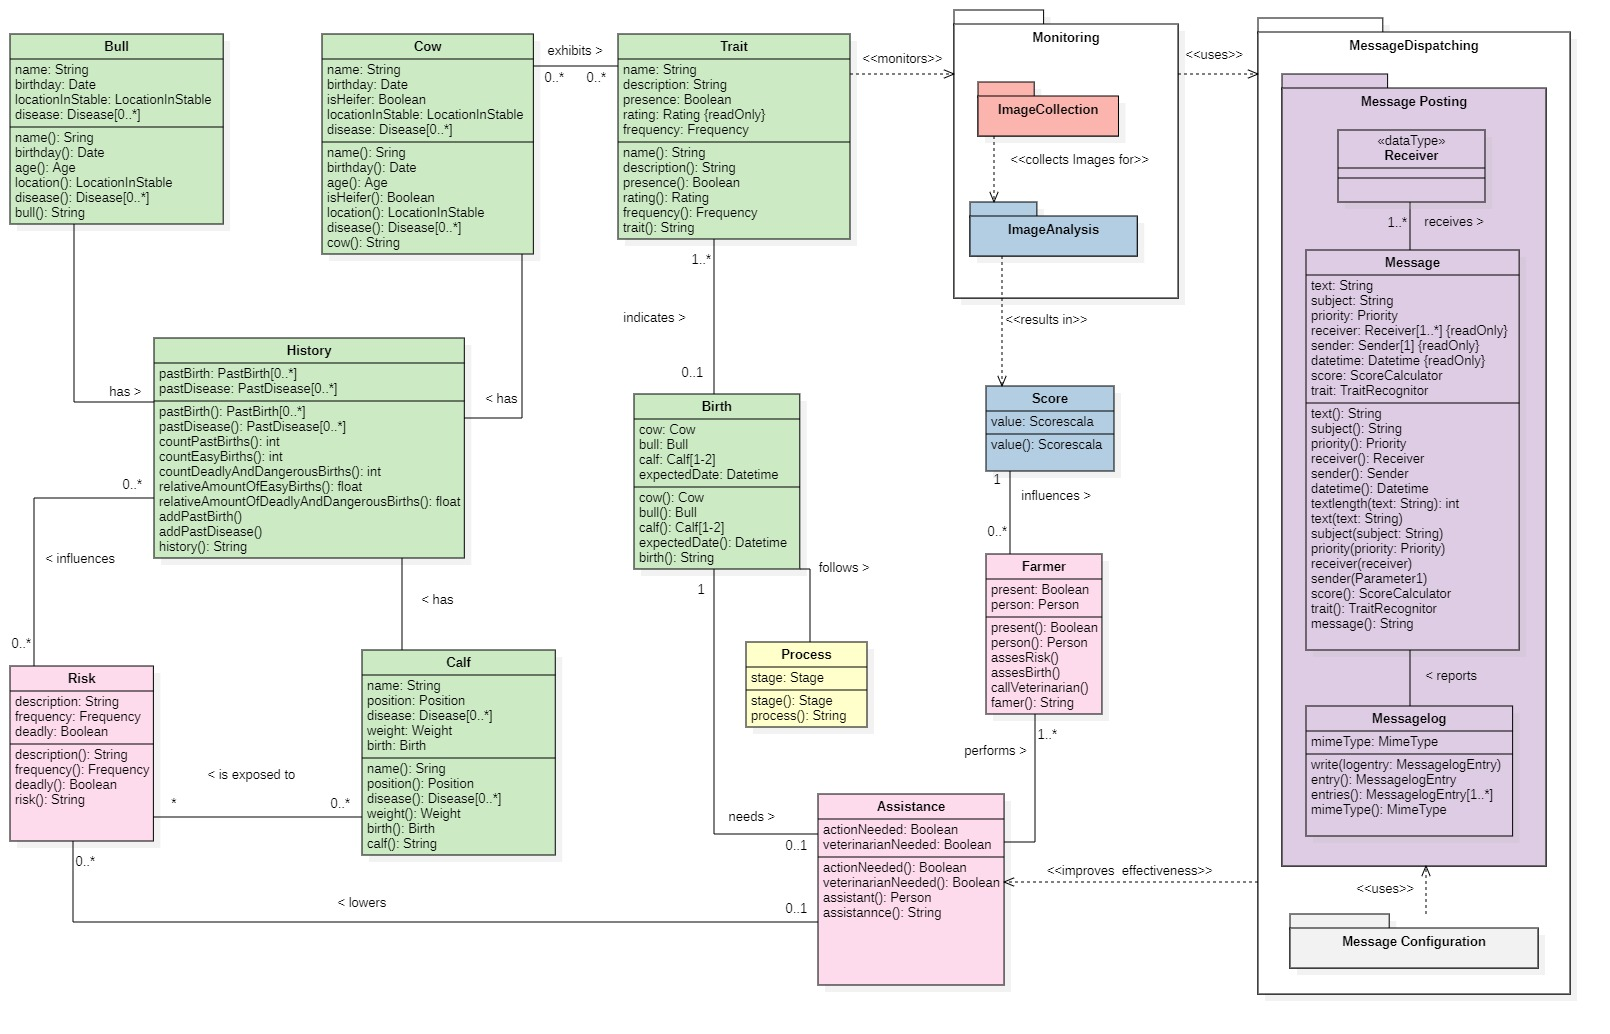
\includegraphics[scale=0.38]{Grafiken/modelle/domain-birth.jpg}
	\caption{Domänenmodell Kalbsgeburt} 
	\label{fig: Domänenmodell Kalbsgeburt}
\end{figure}


\subsection{Allgemeine Bibliothek an Value Objects }


\begin{figure}[H]
	\center
	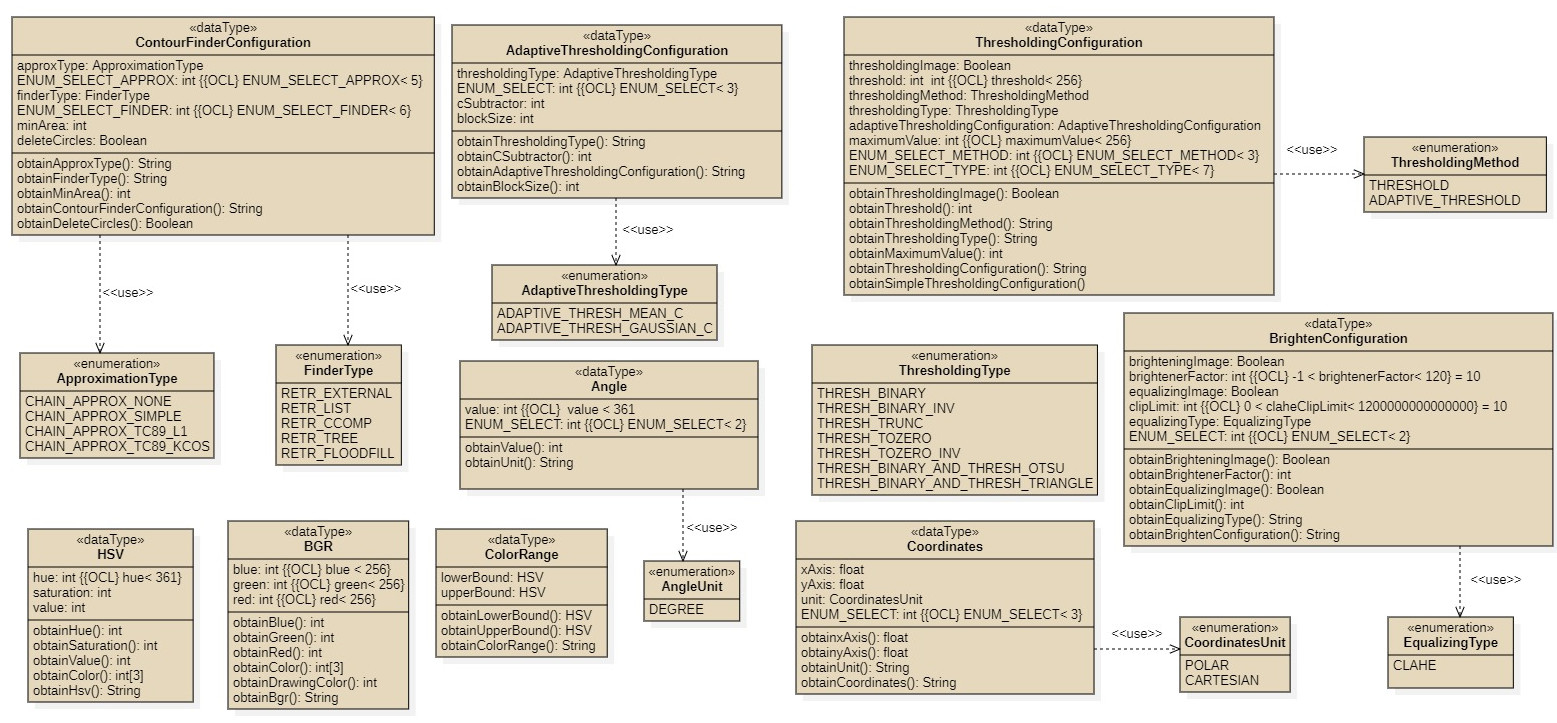
\includegraphics[scale=1.8]{Grafiken/modelle/vo-general2.jpg}
	\caption{Allgemeine Bibliothek an Value Objects}
	\label{fig: Allgemeine Bibliothek an Value Objects} 
\end{figure}

\begin{figure}[H]
	\center
	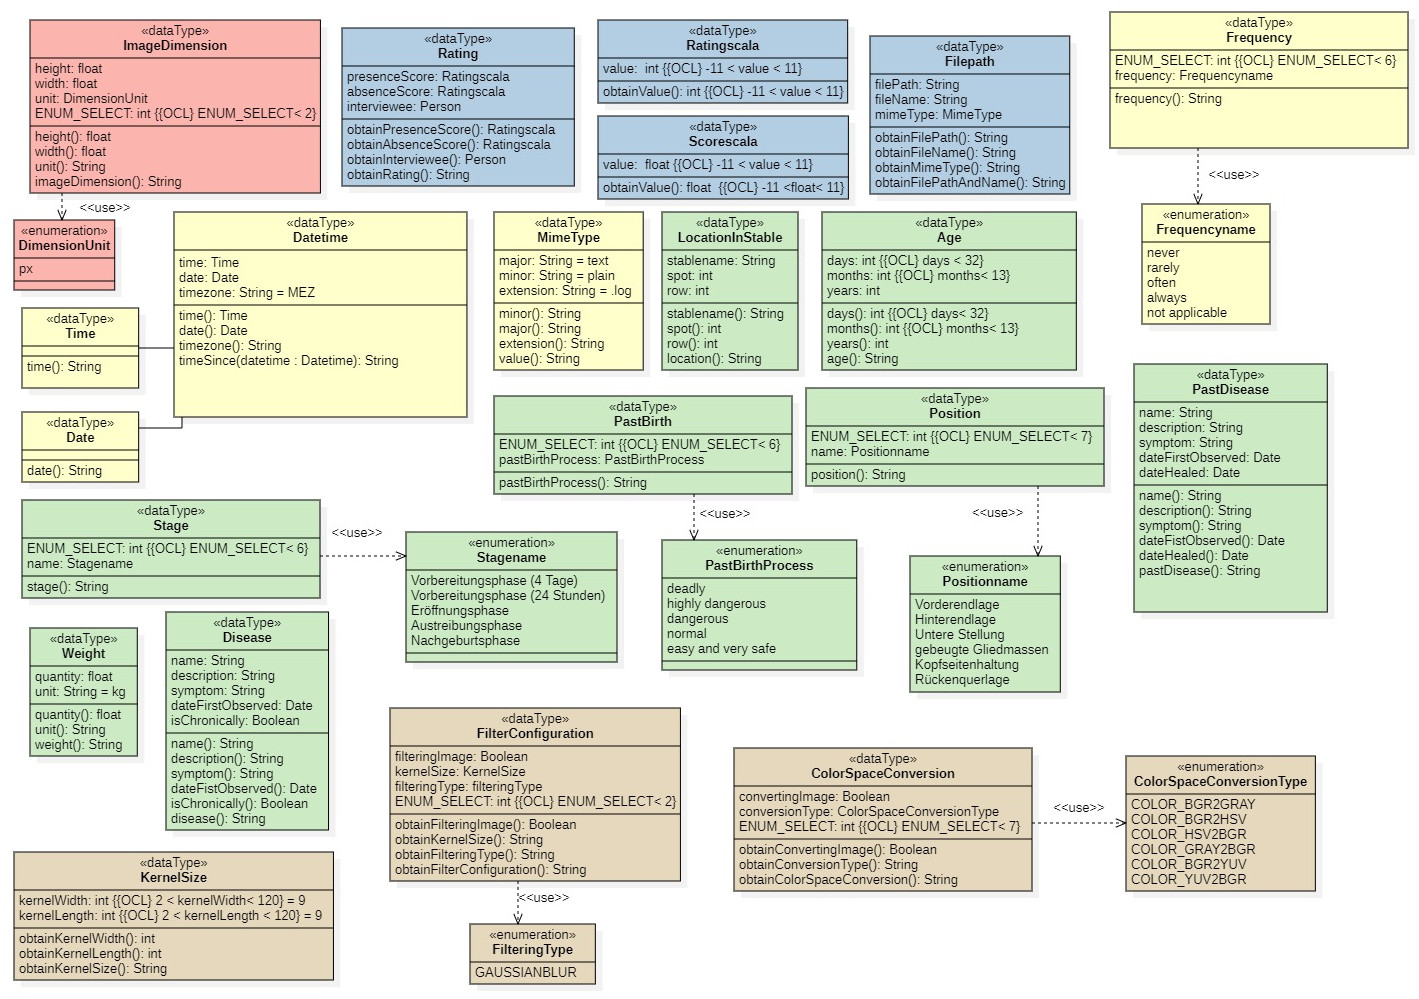
\includegraphics[scale=1.8]{Grafiken/modelle/vo-general1.jpg}
	\caption{Allgemeine Bibliothek an Value Objects  [Fortsetzung]}
	\label{fig: Allgemeine Bibliothek an Value Objects [Fortsetzung]} 
\end{figure}

\subsection{Bibliothek an Value Objects zur Konfiguration und zum Versand von Nachrichten}
\begin{figure}[H]
	\center
	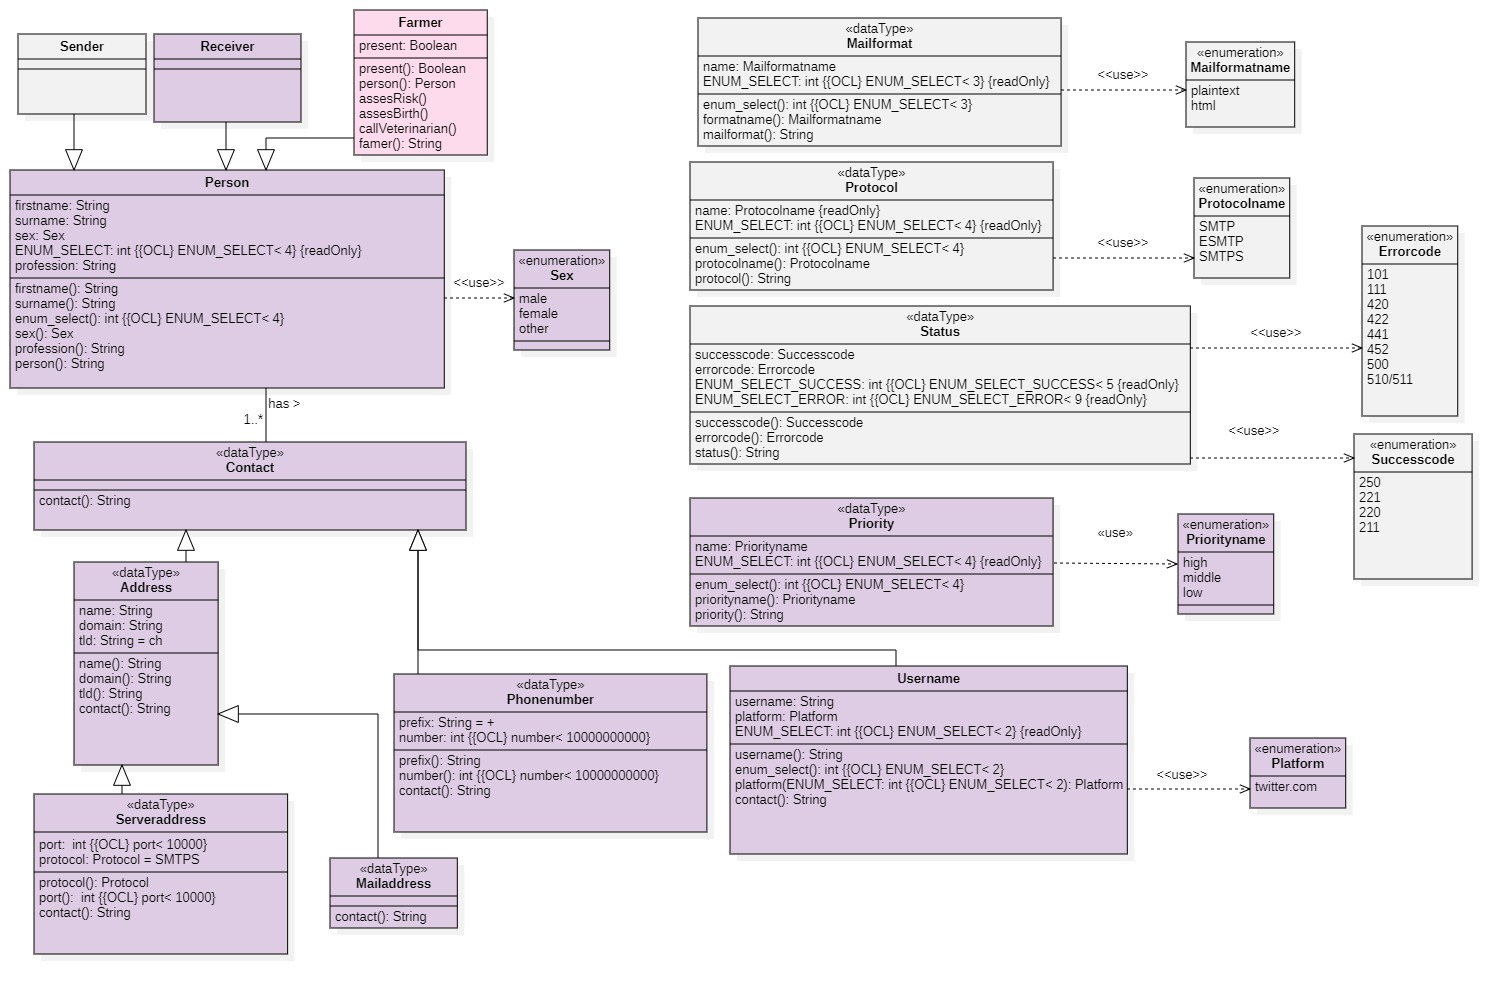
\includegraphics[scale=0.38]{Grafiken/modelle/vo-messaging.jpg}
	\caption{Bibliothek an Value Objects bezüglich Konfiguration und Versand von Nachrichten} 
	\label{fig: Bibliothek an Value Objects zur Konfiguration und zum Versand von Nachrichten}
\end{figure}


\end{landscape}
\restoregeometry % Wieder die alten Ränder